%%\documentclass[12pt,preprint]{aastex}

%% manuscript produces a one-column, double-spaced document:

%\documentclass[manuscript]{aastex}

%% preprint2 produces a double-column, single-spaced document:

 \documentclass[preprint2]{aastex}

%% \documentclass[preprint2,longabstract]{aastex}

\newcommand{\vdag}{(v)^\dagger}
\newcommand{\myemail}{jbyrne@ifa.hawaii.edu}


% ADDING THESE: -JPB
\usepackage{natbib}

\shorttitle{3D CMEs Observed with STEREO}
\shortauthors{Byrne et al.}


\begin{document}

\title{3D Reconstructions of Solar Coronal Mass Ejections Observed During the \emph{STEREO} Mission}

\author{J. P. Byrne$^{1}$, H. Morgan$^{2,3}$, et al.} % P. T. Gallagher$^{4}$, J. M. Refojo$^{5}$, S. R. Habbal$^{1}$}
\affil{$^{1}$Institute for Astronomy, University of Hawai'i, 2680 Woodlawn Drive, Honolulu, HI 96822, USA.\\
	$^{2}$Sefydliad Mathemateg a Ffiseg, Prifysgol Aberystwyth, Ceredigion, Cymru, SY23 3BZ, UK.\\
	$^{3}$Coleg Cymraeg Cenedlaethol, Y Llwyfan, Ffordd y Coleg, Caerfyrddin, Cymru, SA31 3EQ, UK.\\
	$^{4}$School of Physics, Trinity College Dublin, College Green, Dublin 2, Ireland.\\
	$^{5}$Trinity Centre for High Performance Computing, Trinity College Dublin, College Green, Dublin 2, Ireland.
	}


\begin{abstract}
Analysis of numerous CME observations by \emph{STEREO}, via the 3D elliptical tie-pointing reconstruction technique - building on \citet{2010NatCo...1E..74B}.
\end{abstract}

\keywords{Sun: coronal mass ejections (CMEs) --- Methods: miscellaneous --- Techniques: image processing}


\section{Introduction}


\section{Observations}


\section{Elliptical Tie-Pointing Technique}

\subsection{Flux-Rope Model}
\label{fluxropemodel}

A model flux-rope CME is generated, as outlined in \citet{2012ApJ...752..144M}, such that synthetic images can be created for any observer location. This allowed the generation of fits files that correspond to a specified \emph{STEREO} spacecraft separation, for a chosen flux-rope orientation, moving in a given direction away from the Sun. An example of a model flux-rope CME, with orientation normal to the ecliptic ($\zeta = 0^{\circ}$), moving along the Sun-Earth line (latitude $with the \emph{STEREO} spacecraft situated at 90$^{\circ}$ separation.

\begin{figure}[ht]
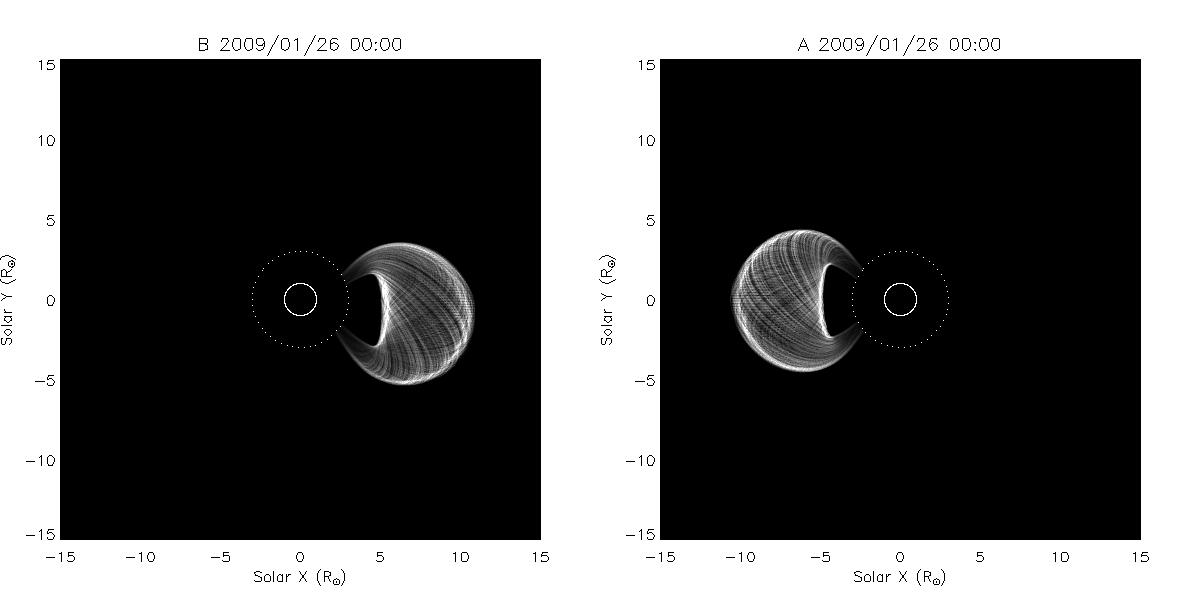
\includegraphics[scale=0.2, trim=0 0 0 0, clip=true]{images/fluxropemodel.jpg}
\caption{Model flux-rope CME}
\label{fluxropemodel}
\end{figure}

\section{Floating material and so forth}


\acknowledgments

This work is supported by SHINE grant 0962716 and NASA grant NNX08AJ07G to the Institute for Astronomy. %The \emph{SOHO}/LASCO data used here are produced by a consortium of the Naval Research Laboratory (USA), Max-Planck-Institut fuer Aeronomie (Germany), Laboratoire d'Astronomie (France), and the University of Birmingham (UK). SOHO is a project of international cooperation between ESA and NASA. \emph{SDO} data supplied courtesy of the NASA/\emph{SDO} consortia.
The \emph{STEREO}/SECCHI project is an international consortium of the Naval Research Laboratory (USA), Lockheed Martin Solar and Astrophysics Lab (USA), NASA Goddard Space Flight Center (USA), Rutherford Appleton Laboratory (UK), University of Birmingham (UK), Max-Planck-Institut f\"{u}r Sonnen-systemforschung (Germany), Centre Spatial de Liege (Belgium), Institut d'Optique Th\'{e}orique et Appliqu\'{e}e (France), and Institut d'Astrophysique Spatiale (France).
%\appendix

%\section{Appendix material}

%For completeness, here is one last equation.
%\begin{equation}
%e = mc^2
%\end{equation}

\bibliographystyle{apj.bst}
\bibliography{references.bib}  


\end{document}